\documentclass[main.tex]{subfiles}

\providecommand{\Par}{\operatorname{Parent}}
\newcommand{\LA}{\operatorname{LA}}
\newcommand{\Dep}{\operatorname{D}}
\newcommand{\LCA}{\operatorname{LCA}}
\newcommand{\argmax}{\operatorname{argmax}}

\begin{document}

\chapter{Ancestors in trees} \label{cap:ancestrais}

\section{Introduction}


Let~$T \coloneqq (V, E)$ be a graph. We say~$T$ is a tree if it is acyclic and connected. In this case, between each pair of vertices in~$T$ there exists a unique path. A tree is rooted when we fix some vertex~${r \in V}$, called the root.

For implementation purposes and without loss of generality, let's assume~$V = \{1, 2, \ldots, |V|\} \eqqcolon [|V|]$.
For each vertex~${u \in V}$, the \deff{ancestors} of~$u$ are the vertices in the (unique) path from~$u$ to~$r$. The~\mbox{$(i-1)$-th} ancestor of~$u$ os the~$i$-th vertex in this path. In particular,~$u$ is the~$0$-th ancestor of~$u$. We say the first ancestor of~$u$, if~$u \neq r$, is the \deff{parent} of~$u$. Define the function~${\Par: V \rightarrow V}$ such that~$\Par(u)$ is the parent of vertex~$u$, for all~$u \in V \setminus \{r\}$; for the vertex~$r$ we can consider that~$\Par(r) = r$. The~\deff{depth} of a vertex~$u$, denoted as~$\Dep(u)$, is the number of edges in the path from~$u$ to~$r$.a

The Level Ancestor problem is the problem of, given~$u \in V$ and~$k \in \mathbb{N}$ such that~$k \leq \Dep(u)$, finding the~$k$-th ancestor of~$u$ , that is, it is the problem of evaluating the function
$$\LA(k, u) \coloneqq \Par^k(u). $$

The Lowest Common Ancestor problem is the problem of, given~$u, v \in V$ , finding the vertex~$w$ with maximum depth that is an ancestor of both~$u$ and~$v$, that is, the problem of evaluating the function
$$\LCA(u, v) \coloneqq \argmax\{\Dep(w) : w \in V,\ w \text{ is an ancestor of $u$ e $v$}\}. $$

\section{Function powers} \label{sec:potfunc}

Let's consider the slightly more generic problem of, given a function~$f: [n] \rightarrow [n]$, which may be represented by an array of size~$n$, build an algorithm that, after some preprocessing over the array~$f$, answers queries of the type: given~$i \in [n]$ and~$k \in [m] \cup \{0\}$, determine~$f^k(i)$ efficiently. If the preprocessing time is~$\Oh(p(n, m))$ and the time to answer each query is~$\Oh(q(n, m))$, we say the complexity of the solution is~$\angles{\Oh(p(n, m)), \Oh(q(n, m))}$.

\subsection{Simple solutions} \label{subsec:anc_sol_simples}

A simple solution is to skip doing any preprocessing, and always do~$k$ iterations to determine~$f^k(i)$. This solution has complexity~$\angles{\Oh(1), \Oh(m)}$. Another simple solution is to store the answer to all possible queries in a matrix~$M$ such that~$M[k][i] = f^k(i)$ for all~$i \in [n]$ and~$k \in [m] \cup \{0\}$. This matrix can be filled using dynamic programming in time~$\Oh(nm)$, since we know that, if~$k > 0$, then~$f^k(i) = f(f^{k-1}(i))$, that is
$$M[k][i] = \left\{
	\begin{array}{ll}
		f(M[k - 1][i]) & \text{ if $k > 0$} \\
		i & \text{ if $k = 0$,}
	\end{array}
	\right.
$$

that is, we can fill~$M$ by iterating through its indices in non-decreasing order relative to~$k$. This solution has complexity~$\angles{\Oh(nm), \Oh(1)}$.

\subsection{Powers of two} \label{subsec:pot2}

The presented simple solutions work in the following way: a base~$(a_1, \ldots, a_x)$ is chosen such that every number between~0 and~$m$ can be written as a sum of zero of more of those numbers, and during preprocessing we caculate~$f^{a_j}(i)$ for all~$i \in [n]$ and~$j \in [x]$. Given a number~$k$, this is written as~${k = a_{b_1} + a_{b_2} + \cdots + a_{b_y}}$ and after that we calculate
$$f^k(i) = f^{a_{b_1}}(f^{a_{b_2}}(\cdots(f^{a_{b_y}}(i))\cdots)).$$
In the first example in Subsection~\ref{subsec:anc_sol_simples} we choose as base only~$(1)$, which makes the query time large, while in the second example we choose~$(1, \ldots, m)$, which makes the preprocessing time large.

If we choose the base more carefully, it's possible to improve the overall complexity. Every integer has a (unique) decomposition as sum of distinct powers of two (corresponding to its binary decomposition), and there are only~$\floor{\lg m}$ powers of two between~1 and~$m$. Therefore, we can choose the base~${(1, 2, 4, \ldots, 2^{\floor{\lg m}})}$. To do the preprocessing, we'll use dynamic programming to fill the matrix~$M$ such that~$M[k][i] \coloneqq f^{2^k}(i)$ for all~$i \in [n]$ and~$0 \leq k \leq \floor{\lg m}$. We know that~$f^x(f^x(i)) = f^{2x}(i)$, so we have that
$$M[k][i] = \left\{
	\begin{array}{ll}
		M[k-1][M[k - 1][i]] & \text{ if $k > 0$} \\
		f(i) & \text{ if $k = 0$,}
	\end{array}
	\right.
$$
and we can fill~$M$ by iterating over its indices in non-decreasing order of~$k$.

\begin{theorem} \label{thm:pot2}
        Every positive integer has an unique decomposition as a sum of distinct powers of two.
\end{theorem}
\begin{proof}
    The proof is by induction. It's obvious that~1 has an unique decomposition.

    Let~$k > 1$ be an integer and let~$2^x$ be the largest power of two that's smaller than or equal to~$k$. Notice that~$k - 2^x < 2^x$ (otherwise~$2^{x+1} \leq k$), so by the induction hypothesis~$k - 2^x$ has an unique decomposition as a sum of distinct powers of two, and none of those are~$2^x$, so we can add this power of two to the representation. This proves existence. Uniqueness follows from the representation of~$k - 2^x$ being unique and, as~$\sum\limits_{0 \leq y < x}{2^{y}} = 2^x - 1 < 2^x \leq k$, we have that any decomposition of~$k$ must contain~$2^x$.
\end{proof}

The proof above gives us an algorithm to find the decomposition of~$k$ as powers of two: it suffices to find the largest power of two which is less than or equal to~$k$, subtract it from~$k$ , and repeat this procedure until~$k$ becomes~0.

\begin{algorithm}
	\caption{Solution for function powers.} \label{lst:potfunclg}
\begin{algorithmic}[1]
	\LineComment{Create matrix~$M$ from~$f$.}
	\Function{Preprocessing}{$f, n, m$}
		\For{$i = 1 \To n$}
			\State $M[0][i] = f(i)$
		\EndFor
		\For{$k = 1 \To \floor{\lg m}$}
			\For{$i = 1 \To n$}
				\State $M[k][i] = M[k - 1][M[k - 1][i]]$
			\EndFor
		\EndFor
	\EndFunction

	\LineComment{Returns~$f^k(i)$; must be called after~\textsc{Preprocessing}.}
	\Function{Query}{$k, i$} \Comment{$k \leq m$ and $i \leq n$}
		\For{$x = \floor{\lg{m}} \DownTo 0$}
			\If{$2^x \leq k$}
				\State $k = k - 2^x$
				\State $i = M[x][i]$
			\EndIf
		\EndFor
		\State \Return $i$
	\EndFunction
\end{algorithmic}
\end{algorithm}

Code listing~\ref{lst:potfunclg} shows the discussed solution, which has time complexity~$\angles{\Oh(n\lg m), \Oh(\lg m)}$ and space complexity~$\Oh(n \lg m)$. Notice that it's easy to implement~\Call{Query}{$k, i$} in a way that it takes~$\Oh(\lg k)$ time; it suffices, in the loop, to start~$x$ with the value of~$\floor{\lg k}$.

\section{Online Level Ancestor for trees}

Since~$\Par$ is a function of~$V$ in~$V$, one can use the algorithms discussed in Section~\ref{sec:potfunc} to evaluate the function~$\LA$. Note that, for each~$u \in V$, we need only compute~$\Par^k(u)$ for~$k < \Dep(u)$, so we use~$n = m = |V|$. These algorithms, however, assume that the function is known beforehand, in order to perform the preprocessing, i.e., the~$\Par$ function must be completely known beforehand (and therefore the tree).

\newcommand{\jmp}{\mathit{jump}}
In Subsection~\ref{subsec:pot2}, we saw that~$M[k][u] = M[k-1][M[k-1][u]]$ can be computed using dynamic programming because it depends on smaller indices of the first coordinate. In the case of trees, however, we know that~$f^{2^{k-1}}(u)$ is an ancestor of~$u$, so to compute the values~$M[k][u]$ for all~${0 \leq k < \floor{\lg \Dep(u)}}$ it suffices that the values of~$M$ are already computed for all ancestors of~$u$, and then we compute~$M[k][u]$ in ascending order of~$k$ (since~$M[k][u]$ depends on~$M[k-1][u]$ in addition to $u$'s ancestors).

For this reason, the algorithm can be implemented online, with new leaves being added to the tree after we already have computed~$M$. To improve the notation in this case, we use at each node an array~$\jmp$ with the values of~$M$, that is,~${u.\jmp[k] = M[k][u] = \Par^{2^k}(u)}$. Once a leaf~$u$ is added, we can compute the values of~$u.\jmp$, in time and space~${\Oh(\floor{\lg \Dep(u)})}$. The query stays the same.

\begin{algorithm}
\caption{Solution for the Level Ancestor problem.} \label{lst:lapot2}
\begin{algorithmic}[1]
	\LineComment{Add the leaf~$u$ to the tree.}
	\Function{\API{AddLeaf}}{$u$}
		\State $u.\jmp[0] = \Par(u)$
		\For{$k = 1 \To \floor{\lg \Dep(u)}$}
			\State $u.\jmp[k] = u.\jmp[k - 1].\jmp[k - 1]$
		\EndFor
	\EndFunction

	\LineComment{Returns~$\LA(k, u)$; must be called after~\funcAPI{AddLeaf}{u}.}
	\Function{\API{LevelAncestor}}{$k, u$}
		\For{$x = \floor{\lg{k}} \DownTo 0$}
			\If{$2^x \leq k$}
				\State $k = k - 2^x$
				\State $u = u.\jmp[x]$
			\EndIf
		\EndFor
		\State \Return $u$
	\EndFunction
\end{algorithmic}
\end{algorithm}

Code listing~\ref{lst:lapot2} solves the online Level Ancestor problem, when you can add leaves to the tree. The operation~$\funcAPI{AddLeaf}{u}$ consumes time~$\Oh(\lg \Dep(u))$ and the operation~$\funcAPI{LevelAncestor}{k, u}$ consumes time~$\Oh(\lg k) = \Oh(\lg \Dep(u))$. Note that each node~$u$ must store an array of size~$\floor{\lg \Dep(u)}$. In the literature, this technique is called Sparse Table, since we ``store'' a table of size~$|V| \times |V|$ by consuming only space~$|V| \lg |V|$, or~Jump Pointers, in this more specific case of the Level Ancestor problem in trees~\cite{BenderM-F2004}. Figure~\ref{fig:treejmppot2} illustrates the jump pointers in a tree.

\begin{figure}[h]
\centering
	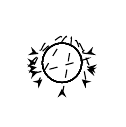
\begin{tikzpicture}[nodes={draw, circle, minimum size=5mm}, sibling distance=25pt, edge from parent/.append style={<-, shorten <= 2pt, shorten >= 2pt}, level distance=35pt]
	\Tree [.\node(v1){}; [.\node(v2){}; [.\node(v3){}; [.\node(v4){}; [.\node(v5){}; ] ] [.\node(v6){}; [.\node(v7){}; ] ] ] [.\node(v8){}; ] [.\node(v9){}; ] ] [.\node(v10){}; [.\node(v11){}; ] ] ]

		\tikzstyle{p2}=[->, shorten >= 2pt, shorten <= 2pt, dashed, >=stealth]
		\tikzstyle{p4}=[->, shorten >= 2pt, shorten <= 2pt, dotted, >=stealth]

		\draw[p2] (v3) edge[out=90,in=180] (v1);
		\draw[p2] (v4) edge[out=10,in=200] (v2);
		\draw[p2] (v5) edge[out=130,in=190] (v3);
		\draw[p4] (v5) edge[out=150,in=160] (v1);
		\draw[p2] (v8) edge[out=70,in=270] (v1);
		\draw[p2] (v9) edge[out=60,in=-40] (v1);
		\draw[p2] (v11) edge[out=30,in=20] (v1);
		\draw[p4] (v7) edge[out=0,in=-10] (v1);
		\draw[p2] (v6) edge[out=80,in=220] (v2);
		\draw[p2] (v7) edge[out=50,in=-15] (v3);
\end{tikzpicture}
	\caption{Example of a tree with jump pointers. The filled edges are parent edges~($\jmp[0]$), the dashed edges skip two levels~($\jmp[1]$), and the dotted edges skip four levels~($\jmp[2]$).} \label{fig:treejmppot2}
\end{figure}

\section{Lowest Common Ancestor} \label{sec:lca_pot2}

\newcommand{\kb}{k^\star}

Let~$u, v \in V$ and~$c \in V$ be the lowest common ancestor of~$u$ and~$v$. Suppose, without loss of generality, that~${\Dep(v) \geq \Dep(u)}$. It is obvious that~${\Dep(c) \leq \Dep(u)}$, so we can ``level'' the vertices~$u$ and~$v$, i.e., exchange~$v$ for~${\LA(\Dep(v) - \Dep(u), v)}$.
Thus, we can assume that~$\Dep(u) = \Dep(v)$ and, to find the lowest common ancestor of~$u$ and~$v$, we must find the smallest~$\kb$ such that~${\LA(\kb, u) = \LA(\kb, v)}$. Note that if~${k < \Dep(u) - 1}$ and~${\LA(k, u) = \LA(k, v)}$, then
$${\LA(k + 1, u) = \Par(\LA(k, u)) = \Par(\LA(k, v)) = \LA(k + 1, v).}$$
This will allow the jump pointers to be used to determine such minimal~$\kb$.

If~${x < \kb}$ then~${\LA(x, u) \neq \LA(x, v)}$, that is, we have a way to check whether~$x < \kb$ without knowing~$\kb$. Just like in the proof of Theorem~\ref{thm:pot2}, to decompose a number as a sum of distinct powers of two, we simply determine the greatest power of two less than or equal to that number, add it to the decomposition, and repeat. Since we have jump pointers to the powers of two for all nodes, we can determine the decomposition as a sum of powers of two for~${\kb - 1}$ (since we can test~${x \leq \kb - 1}$ and not~${x \leq \kb}$), and similarly to the function~\API{LevelAncestor} of Code listing~\ref{lst: lapot2}, we can determine the~\mbox{$(\kb-1)$-th} ancestor of~$u$ and~$v$ in time~$\Oh(\lg \Dep(u))$.


\begin{algorithm}
\caption{Lowest Common Ancestor using Jump Pointers. \label{lst:lcapot2}}
\begin{algorithmic}[1]
	\Function{\API{LowestCommonAncestor}}{$u, v$}
		\If{$\Dep(u) > \Dep(v)$}
			\State $u, v = v, u$ \Comment{Guarantees that~$\Dep(u) \leq \Dep(v)$.}
		\EndIf
		\State $v = \funcAPI{LevelAncestor}{\Dep(v) - \Dep(u), v}$ \Comment{Levels~$v$.}
		\If{$u = v$} \label{lst:lcapot2:if2}
			\State \Return $u$
		\EndIf
		\For{$i = \floor{\lg \Dep(u)} \DownTo 0$} \label{lst:lcapot2:for}
			\If{$u.\jmp[i] \neq v.\jmp[i]$} \label{lst:lcapot2:iffor}
				\State $u = u.\jmp[i]$
				\State $v = v.\jmp[i]$
			\EndIf
		\EndFor
		\LineComment{$u$ is now a child of the LCA between~$u$ and~$v$.}
		\State \Return $\Par(u)$
	\EndFunction
\end{algorithmic}
\end{algorithm}

\begin{invar}
At the start of the iteration with value~$i$ of the~\keyword{for} of the~\nref{lst:lcapot2:for}-th line of Code listing~\ref{lst:lcapot2}, it holds that~${0 < \Dep(u) - \Dep(c) \leq 2^{i+1}}$, where~${c = \LCA(u, v)}$, and the value of~$\LCA(u, v)$ does not change at the end of the iteration.
\end{invar}
\begin{proof}
	For the base,~$i = \floor{\lg\Dep(u)}$ and
	$$\Dep(u) - \Dep(c) \leq \Dep(u) = 2^{\lg\Dep(u)} \leq 2^{\floor{\lg\Dep(u)}+1}.$$
	Furthermore, if~$u = c$, then the~\keyword{if} of line~\nref{lst:lcapot2:if2} is executed, thus~${\Dep(u) - \Dep(c) > 0}$..

	Suppose that the invariant holds at the beginning of the iteration with value~$i$, and we will prove that it continues to hold at the beginning of the iteration with value~$i - 1$. Let~${d \coloneqq \Dep(u) - \Dep(c)}$. We then know that~${0 < d \leq 2^{i+1}}$. Note that~${d \leq 2^i}$ if and only if ${\LA(2^i, u) = \LA(2^i, v)}$, i.e., the~\keyword{if} of the line~\nref{lst:lcapot2:iffor} is executed if and only if~$d > 2^i$. So
	\begin{itemize}
		\item if~$d \leq 2^i$, the invariant already holds for~$i-1$ and the~\keyword{if} is not executed;
		\item if~$d > 2^i$, the~\keyword{if} is executed, so we exchange~$u$ for~$\LA(2^i, u)$ and~$v$ for~$\LA(2^i, v)$. Let~$d'$ be the new value of~$\Dep(u) - \Dep(c)$. The depth of both~$u$ and~$v$ decrease by~$2^i$, thus~$$d' = d - 2^i \leq 2^{i+1} - 2^i = 2^i.$$
		Since~$d > 2^i$, we also have that~${d' = d - 2^i > 0}$, so the invariant still holds.
	\end{itemize}
\end{proof}

Therefore, at the end of the last iteration, the invariant holds for~$i = -1$, i.e., it holds that~${0 < \Dep(u) - \Dep(c) \leq 2^0 = 1}$, so~$c$ is the parent of~$u$ and the function returns the correct value.

Table~\ref{tab:la_pot2} shows the time and space complexity of the implementations discussed in this chapter.

A Tabela~\ref{tab:la_pot2} mostra o consumo de tempo e espaço das implementações discutidas nesse capítulo.

\begin{table}[h] \centering
\begin{tabular}{|l|c|}
	\hline
	Function & Time/Space \\ \hline
	\funcAPI{AddLeaf}{u} & $\Oh(\lg n) / \Oh(\lg n)$ \\
	\funcAPI{LevelAncestor}{k, u} & $\Oh(\lg n) $ \\
	\funcAPI{LowestCommonAncestor}{u, v} & $\Oh(\lg n)$ \\ \hline
\end{tabular}
	\caption{Time and Space complexity of the discussed solution, where~$n$ is the size of the tree.} \label{tab:la_pot2}
\end{table}

\end{document}
